\documentclass{article}
\usepackage{amsmath, amssymb,amsfonts,tikz, mdframed,mathtools}
\usetikzlibrary{shapes,arrows,calc,positioning,backgrounds}
\title{Algorithms \& Complexity: Lecture 2, Time and space complexity}
\author{Sam Barrett}

\newmdtheoremenv{thesis}{Thesis}
\newmdtheoremenv{problem}{Problem}
\newmdtheoremenv{proof}{Proof}

\newcommand{\N}{\mathbb{N}}
\newcommand\defeq{\stackrel{\mathclap{\normalfont\mbox{def}}}{=}}

\begin{document}

\maketitle

\section{Upper and lower bounds}

A simple set of examples for upper and lower bounds could be:

\begin{itemize}
  \item \textbf{Upper bound:} I can clear my flat in a couple of days at most.
  \item \textbf{Lower bound:} It will take me at least a day to clear my flat.
\end{itemize}

\subsection{Upper bound notation}

\textbf{Note:} this notation is not \underline{only} used for time complexity.

Say that we have two functions: $f: \N \rightarrow \N$ and $ g: \N \rightarrow \N$.

We say that $f(n)$ is $O(g(n))$ if $f$ is \textbf{no bigger} than $g$ up to a constant factor. Or more precisely, if there are numbers $c$ and $n_{o}$ such that, $\forall n, n \geq n_{0}$ we have $f(n) \leq c \cdot g(n)$.

\underline{Example}

\[
  f(n) \leq 15n^{3}, \forall n \geq 1000
\]

In this situation we can say that $f(n)$ is $O(n^{3})$.

We have:
\begin{itemize}
  \item $c =15$
  \item $n_{0} = 1000$
  \item $g(n) = n^{3}$
\end{itemize}


We say that $f(n)$ is $o(g(n))$ if $f$ is not as big as $g$, even up to any constant factor. Or more precisely, if, for any $\epsilon > 0$, there is $n_{0}$ such that, $\forall n \geq n_{0} $ we have $f(n) \leq \epsilon \cdot g(n)$

We can therefore see, if $f(n)$ is $o(g(n))$ then $f(n)$ is always also $O(g(n))$ this can be proven if you take $c$ to be 1.

\subsubsection{Examples}

\underline{Example 1}

$  5n^{2} + 17n + 3$ is $O(n^{2})$ and $o(n^{3})$ and $O(n^{3})$ but \textbf{not} $o(n^{2})$.

\begin{itemize}
  \item This is the case as we it is clearly no bigger than $O(n^{2})$ (up to a constant factor) as it contains a quadratic term.
  \item It is \textit{small} compared with $n^{3}$ (hence $o(n^{3})$) as the highest factor again is $n^{2}$.
  \item It is also $O(n^{3})$ as if it is no bigger than $O(n^{2})$ it follows that it must also be no bigger than $O(n^{3})$.
  \item We cannot, however, say that it is $o(n^{2})$ as it cannot be smaller than $n^{2}$ due to it containing a quadratic term.
\end{itemize}

\underline{Example 2}

$8n\log n$ is $O(n\log n)$ and $o(n^{2})$

We can say this as:

\begin{itemize}
  \item our term cannot be any bigger than $n\log n$ (up to a constant factor)
        \item It must be smaller than $n^{2}$, due to the nature of logarithms.
\end{itemize}

\subsection{Lower bound notation}

\begin{itemize}
  \item We say that $f(n)$ is $\Omega(g(n))$ when $g(n)$ is $O(f(n))$

        Meaning, there $c$ and $n_{0}$ such that, $\forall n \geq n_{0}$ we have $f(n) \geq c \cdot g(n)$
  \item We say that $f(n)$ is $\omega(g(n))$ when $g(n)$ is $o(f(n))$
  \item We say that $f(n)$ is $\Theta(g(n))$ when it is both $O(g(n))$ and $\Omega(g(n))$

        Informally we say this means: ``$f(n)$ and $g(n)$ are the same, up to a constant factor''
\end{itemize}


\section{Time complexity}

\subsection{Running time for a machine $M$}

The running time of a machine $M$ is the time taken from the input state, where $x$ sits on the input tape and the other tapes are blank, to reach the halt state ($q_{\texttt{halt} }$).

For any number $n$, we defien $\texttt{WT}_{M}(n) $ to be the \textbf{worst case} running time for an input of length $n$.
For example,

\begin{center}
 \begin{tabular}{|c|c|}
 \hline
 Input & Running time\\ [0.5ex]
 \hline\hline
 00 & 15 \\
 \hline
 01 & 23 \\
 \hline
 10 & 7 \\
 \hline
 11 & 12\\
 \hline
\end{tabular}
\end{center}

Here $\texttt{WT} _{M}(2) = 23$. If we were to say that $\texttt{WT} _{M}(n)$ is $O(n^{2})$ we are saying that there are numbers $n_{0}$ and $C$ such that, $\forall n \geq n_{0}$, the running time is $\leq Cn^{2}$.

\subsection{\texttt{DTIME} classes }

$\texttt{DTIME}(n^{2})$ is a \textbf{complexity class}, a complexity class can be thought of as a set of decision problems.

A decision problem, $f : \{ 0,1 \}^{*} \rightarrow \{ 0,1 \}  $ is in $\texttt{DTIME}(n^{2}) $ when there is some machine (of any sized alphabet or number of tapes) that decides it ($f$) and has worst case running time in $O(n^{2})$.

\subsubsection{Example: palindromes}

We can again define our set $\texttt{PAL} $ of all palindromic bitstrings with a boolean function $f: \{ 0,1 \}^{*}\rightarrow \{ 0,1 \} $.

Given we have a machine $A-B$ which utilises 3 tapes to decide \textit{palindromicity}  and has worst case running time $O(n)$. We can therefore say that $\texttt{PAL} $ is in $\texttt{DTIME} (n)$.

Can this be improved upon?

\textbf{No!} This can be trivially explained as any solution to palindromicity \textbf{must} at least read the input string of length $n$, therefore there must be \textbf{at least} $n$ steps to the computation, leading to a best case running time in $\Omega(n)$.

\subsection{Polynomial time}

We can define the complexity (super) class of \textbf{polynomial time decision problems} as:

\[
  P \;\; \defeq \;\; \bigcup_{k\geq1}\texttt{DTIME} (n^{k})
\]

From this definition, you can see that \textbf{any} decision problem in $\{  \texttt{DTIME} (n^{k})\}_{k=0}^{\infty} $ is also in $P$

\subsubsection{Robustness}

Is this definition robust?

\begin{itemize}
  \item Converting a large alphabet into our default alphabet ($\{ \rhd, \Box, 0,1 \} $) only multiplies the running time by a constant factor
  \item Converting a $n$ tape machine to a 3,2 or 1 tape machine \textbf{squares} the running time. This is more significant
  \item Converting a machine whose tapes are infinite in both directions to a machine whose tapes are infinite in only one direction multiplies the running time by a constant factor
        \item Converting a machine whose tapes are 2 dimensional to a machine whose tapes are one dimensional \textbf{squares the running time}. This is more significant.
\end{itemize}

In \textbf{all} of the cases listed above, the notion of polynomial time that you are left with is the \textbf{same}. The same class of decision problems are solvable in polynomial time.

\textbf{Note: this is true for polynomial time (as defined above) but is not the case for linear or quadratic time }

For example, \texttt{PAL} can be solved in $O(n)$ on a multitape Turing machine but is $\Theta(n^{2})$ on a single tape machine.

\subsubsection{Size of input}

Another common concern is that our data may be represented as a bitstring in more than one way. However, in practical examples, the representations differ by a \textbf{constant} factor leading to polynomial time being the same.

\subsection{Exponential time}

We can define the complexity class of \textbf{exponential time decision problems as}:

\[
  \texttt{EXP} \;\;\; \defeq \;\;\; \bigcup_{k\geq 1 }\texttt{DTIME} (2^{n^{k}})
\]

Therefore, any decision problem in $\texttt{DTIME} (2^{5n^{17}})$ is in $\texttt{EXP} $ and so on.

Also clearly $P \subseteq \texttt{EXP} $

\section{Space complexity}

Although we often regard time complexity as being the most important, there are many cases in which we need to worry about space complexity as well.

\subsection{Space usage of a machine $M$}

The \textbf{space usage} for an input $x$ is the number of cells on the \textbf{work tapes} that are non-blank at some point during execution.

\textbf{We ignore blank cells as at any point in computation there are infinitely many of these}

For any number $n$ we define $\texttt{WS}_{M}(n)$ to be the worst case space usage for an input of length $n$.

For example:

\begin{center}
 \begin{tabular}{|c|c|}
 \hline
 Input & Space usage \\ [0.5ex]
 \hline\hline
 00 & 5 \\
 \hline
 01 & 12 \\
 \hline
 10 & 9 \\
 \hline
 11 & 9\\
 \hline
\end{tabular}
\end{center}

Here $\texttt{WS}_{M}(2) = 12 $. Saying that $\texttt{WS}_{M}(n) $ is $O(n^{2})$ means that there are numbers $n_{0}$ and $C$ such that, $\forall n \geq n_{0}$, the space usage is $\leq Cn^{2}$.

\underline{Example execution}

\textbf{Input tape:}
\begin{center}

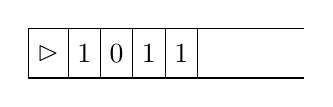
\begin{tikzpicture}[
block/.style={minimum height=1.8em,outer sep=0pt,draw,rectangle,node distance=0pt}]

        \node [block] (A) {$\rhd$};
        \node [block, right = of A] (B) {1};
        \node [block, right = of B] (C) {0};
        \node [block, right = of C] (D) {1};
        \node [block, right = of D] (E) {1};

        \draw (A.north east) -- ++(3cm,0) (A.south east) -- ++ (3cm,0);
    \end{tikzpicture}

\end{center}

A key point about the calculation of space usage is that we \textbf{do not} count the number of non-blank cells on the input tape, only on the work tapes.

\textbf{Work tape 1:}
\begin{center}

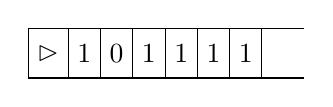
\begin{tikzpicture}[
block/.style={minimum height=1.8em,outer sep=0pt,draw,rectangle,node distance=0pt}]


        \node [block] (A) {$\rhd$};
        \node [block, right = of A] (B) {1};
        \node [block, right = of B] (C) {0};
        \node [block, right = of C] (D) {1};
        \node [block, right = of D] (E) {1};
        \node [block, right = of E] (F) {1};
        \node [block, right = of F] (G) {1};
        \draw (A.north east) -- ++(3cm,0) (A.south east) -- ++ (3cm,0);
    \end{tikzpicture}

\end{center}

  \textbf{Work tape 2:}
  \begin{center}

    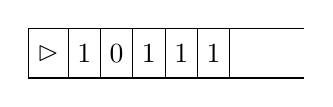
\begin{tikzpicture}[
    block/.style={minimum height=1.8em,outer sep=0pt,draw,rectangle,node distance=0pt}]


        \node [block] (A) {$\rhd$};
        \node [block, right = of A] (B) {1};
        \node [block, right = of B] (C) {0};
        \node [block, right = of C] (D) {1};
        \node [block, right = of D] (E) {1};
        \node [block, right = of E] (F) {1};

          \draw (A.north east) -- ++(3cm,0) (A.south east) -- ++ (3cm,0);
        \end{tikzpicture}


  \end{center}

  The space usage above would be 11.

  \subsection{\texttt{SPACE} complexity class}

  $\texttt{SPACE} (n^{2})$ is a complexity class and a decision problem $f: \{ 0,1 \}^{*} \rightarrow \{ 0,1 \}  $ is in this space when there is some machine (with any size of alphabet or number of tapes) that decides it ($f$) and has a worst case space usage in $O(n^{2})$


  \subsection{\texttt{L} and \texttt{PSPACE} }

  We can now define logarithmic space ($\texttt{L} $) which defines the set of things that can be computed with a machine using a logarithmic number of cells

  \textbf{Note: this relies on the fact that we do not count the number of cells on the input tape.} This is because if we were to count the input tape there would be at least $n$ cells used and $n > \log n$, similarly to how we cannot have \texttt{PAL} solved in less than linear time.

  \[
    \texttt{L}  \;\;\; \defeq  \;\;\; \texttt{SPACE}(\log n)
  \]

  We can also define polynomial space $\texttt{PSPACE} $

  \[
    \texttt{PSPACE} \;\;\; \defeq \;\;\; \bigcup_{k\geq1} \texttt{SPACE} (n^{k})
  \]

  It is also clear taht $\texttt{L} \subseteq \texttt{PSPACE} $

  \subsubsection{Robustness}

  Is this robust?

  Yes, it is in fact more simple than with time.

  \begin{itemize}
    \item Converting a large alphabet into our default alphabet ($\{ \rhd, \Box, 0,1 \} $) only multiplies the space usage by a constant factor

    \item Converting a $n$ tape machine to a 3,2 or 1 tape machine multiplies space usage by a constant factor.

    \item Converting a machine whose tapes are infinite in both directions to a machine whose tapes are infinite in only one direction multiplies the space usage by a constant factor

    \item Converting a machine whose tapes are 2 dimensional to a machine whose tapes are one dimensional multiplies space usage by a constant factor.

  \end{itemize}

  In all of these cases, logarithmic space does not depend on the model.

  \subsection{Space vs time}

  We can show that in all cases, space complexity is less or equal to time complexity.

  We can prove by example that $\texttt{P} \subseteq \texttt{PSPACE} $:

  \begin{itemize}
    \item Let $M$ be a machine with 5 work tapes that, for any input of length $n \geq 1000$, has a running time of $\leq 18n^{3}$ steps (a poly-time machine).
    \item For such an input, the space used is at most $5+5\times 18n^{3}$

          This is true as 5 cells are non-blank initially  and at most 5 more cells per step of execution ($5 \times \texttt{steps}$) $\implies 5 + (5 \times 18n^{3})$
  \end{itemize}

  We can also how that, in all cases, time is less than or equal to exponentiated space.
  The following is a proof of $\texttt{L} \subseteq P $

  \begin{itemize}
    \item Let $M$ be a machine with 5 work tapes, 74 states 13 symbols and it eventually halts, that, for any input of length $n\geq 1000$ has a space usage of $\leq 18\log n$ cells

    \item For such an input, the number of \textbf{configurations} is at most

          \[
          74 \times 13^{18\log n} \times (18\log n)^{5}\times (n+2)
          \]

          Where a \textbf{configuration} tells us everything about the machine at a given point in execution
          \begin{itemize}
            \item the state
            \item what is written on each work tape
            \item where the head is on each work tape
            \item where the head is on the input tape
          \end{itemize}

          and

          \begin{itemize}
            \item 74 is the number of states in which the following apply
            \item $13^{18\log n}$ is the number of possible symbols in each of the maximum number of memory cells
            \item $(18\log n)^{5}$ represents all the possible head locations over the 5 tapes
            \item On the input tape we have $n+2$ cells in use. This is due to it containing the start symbol $\rhd$, $n$ bits and a single blank cell.
          \end{itemize}

          We can also see that this number of configurations in bounded by a polynomial as its constituent parts are bounded by polynomials ($\log$ etc.).

          The execution time cannot be greater than this because that would mean some configuration is repeated, causing an infinite loop. This is the case as if we reach the same configuration for a second time, there is nothing to prevent it from simply repeating everything it did subsequent to the last time it was in that configuration, thus looping. This cannot be the case as we have assumed our machine $M$ to halt.

  \end{itemize}

  Therefore, if the space usage is logarithmic, the running time is polynomial.

  The same argument can be made to show that if we have something in polynomial \textbf{space} it must be in \textbf{exponential } time. To construct this proof simply replace the $\log n$ in the above proof with a polynomial.


\section{Nondeterministic time complexity}

\section{Nondeterministic space complexity}

\end{document}
